\section{Higgs Properties}
\label{sec:properties}

With the announcement of the discovery of a new state near 125 GeV, attention at ATLAS and CMS 
turned to the characterization of the particle through  measurements of its properties. 
In particular, emphasis is placed on ascertaining the compatibility 
of the new state with the SM Higgs boson.
This section includes discussions of some of the techniques used at CMS to determine the properties 
of the newly discovered state and results presented at the HCP symposium in November 2012. 
All of the analyses described in Section~\ref{sec:combinedsearchresults},
with exception of $\Hgg$, were updated to improve their sensitivity 
and include the additional data collected at CMS~\citep{HIG-12-045}. The total integrated 
luminosity of the 8 TeV data sample used is up to $12.2 fb^{-1}$ depending on the
specific channel.

\subsection{Extracting Signal Parameters}

The best fit value for the signal strength is evaluated 
by scanning for the value of $\mu$ at which the likelihood (Equation~\ref{eqn:likelihood})
attains its maximum in data. This can be extended where more than one signal parameter
is of interest by generalising to the profiled likelihood ratio,
\begin{equation}
q_{\boldmu} = 
	-2\ln\frac{\displaystyle \mathcal{L}(data | \mu,\hat{\boldth}_{\boldmu})}
	{\displaystyle \mathcal{L}(data | \hat{\boldmu},\hat{\boldth})}, 
\label{eqn:llrNd}
\end{equation}
where $\boldmu=x_{1},x_{2},\cdots$$,x_{N}$ represents the $N$ parameters
of interest in the signal model. The values of the nuisance parameters 
which maximise the value of the likelihood first 
fixing the values of $\mu$ and then letting them float freely are
denoted $\hat{\boldth}_{\boldmu}$ and $\hat{\boldth}$ respectively.
The values for which $q_{\boldmu}=0$ in the observed data are the best fit values.
The contour defined by the set of points for which $C_{N}(q_{\boldmu})=0.68$,
where $C_{N}$ is the cumulative distribution function (cdf) of a chi-squared distribution
with $N$ degrees of freedom, is interpreted
as the 68\% confidence contour. In one dimension, the values at which $q_{\boldmu}=1$
represent the usual 68\% confidence interval.
This method for extracting confidence intervals is known to fail when the best fit 
values lie within or near non-physical regions.
It is necessary therefore to cross-check this method to avoid quoting
non-physical results. This is achieved through the use of the Feldman-Cousins procedure.

\subsubsection{The Feldman-Cousins Procedure for Evaluating Confidence Intervals}

For parameters such as the relative production cross-section, $\mu$, negative values 
are not considered physical. Constraints on the fit can be imposed to avoid quoting unphysical values. 
However, where the best-fit values for the signal model parameters lie outside physically
allowed regions, the relationship between the values of $q_\mu$ and
the 68\% confidence interval no longer holds. 
In order to assign the correct confidence intervals, the Feldman-Cousins
procedure is used~\citep{fc}.  
The procedure involves throwing pseudo-datasets and evaluating 
a test-statistic to determine the compatibility of the data with each 
point in the $N$-dimensional parameter space.
The test-statistic used in the one-dimensional case of the signal strength
is defined using the ratio of profiled likelihoods, $\qmu$ (Equation~\ref{eqn:llr2}).
The physical constraint on the parameter is imposed in this case by 
requiring that $\hat{\mu} \ge 0$. 
The probability to obtain a value of the test-statistic larger than the one 
observed in data ($CL_{s+b}$) is calculated as in Equation~\ref{eqn:clsplusb},
where the distribution $f(\qmu | \mu,\boldth=\boldth_{\mu}^{obs})$ is 
generated from evaluating the test-statistic in pseudo-datasets. 
As with calculating upper limits, for generating the pseudo-data, the nuisances ($\boldth$) 
are set to the values obtained from a fit to the data.
Figure~\ref{fig:fcegtoys} shows an example of this distribution for two 
values of $\mu$ from the (0/1)-jet bin of the $\Htt$ analysis and the values of 
$q_\mu^{obs}$ obtained from the observed data.
\begin{figure}
\begin{center}
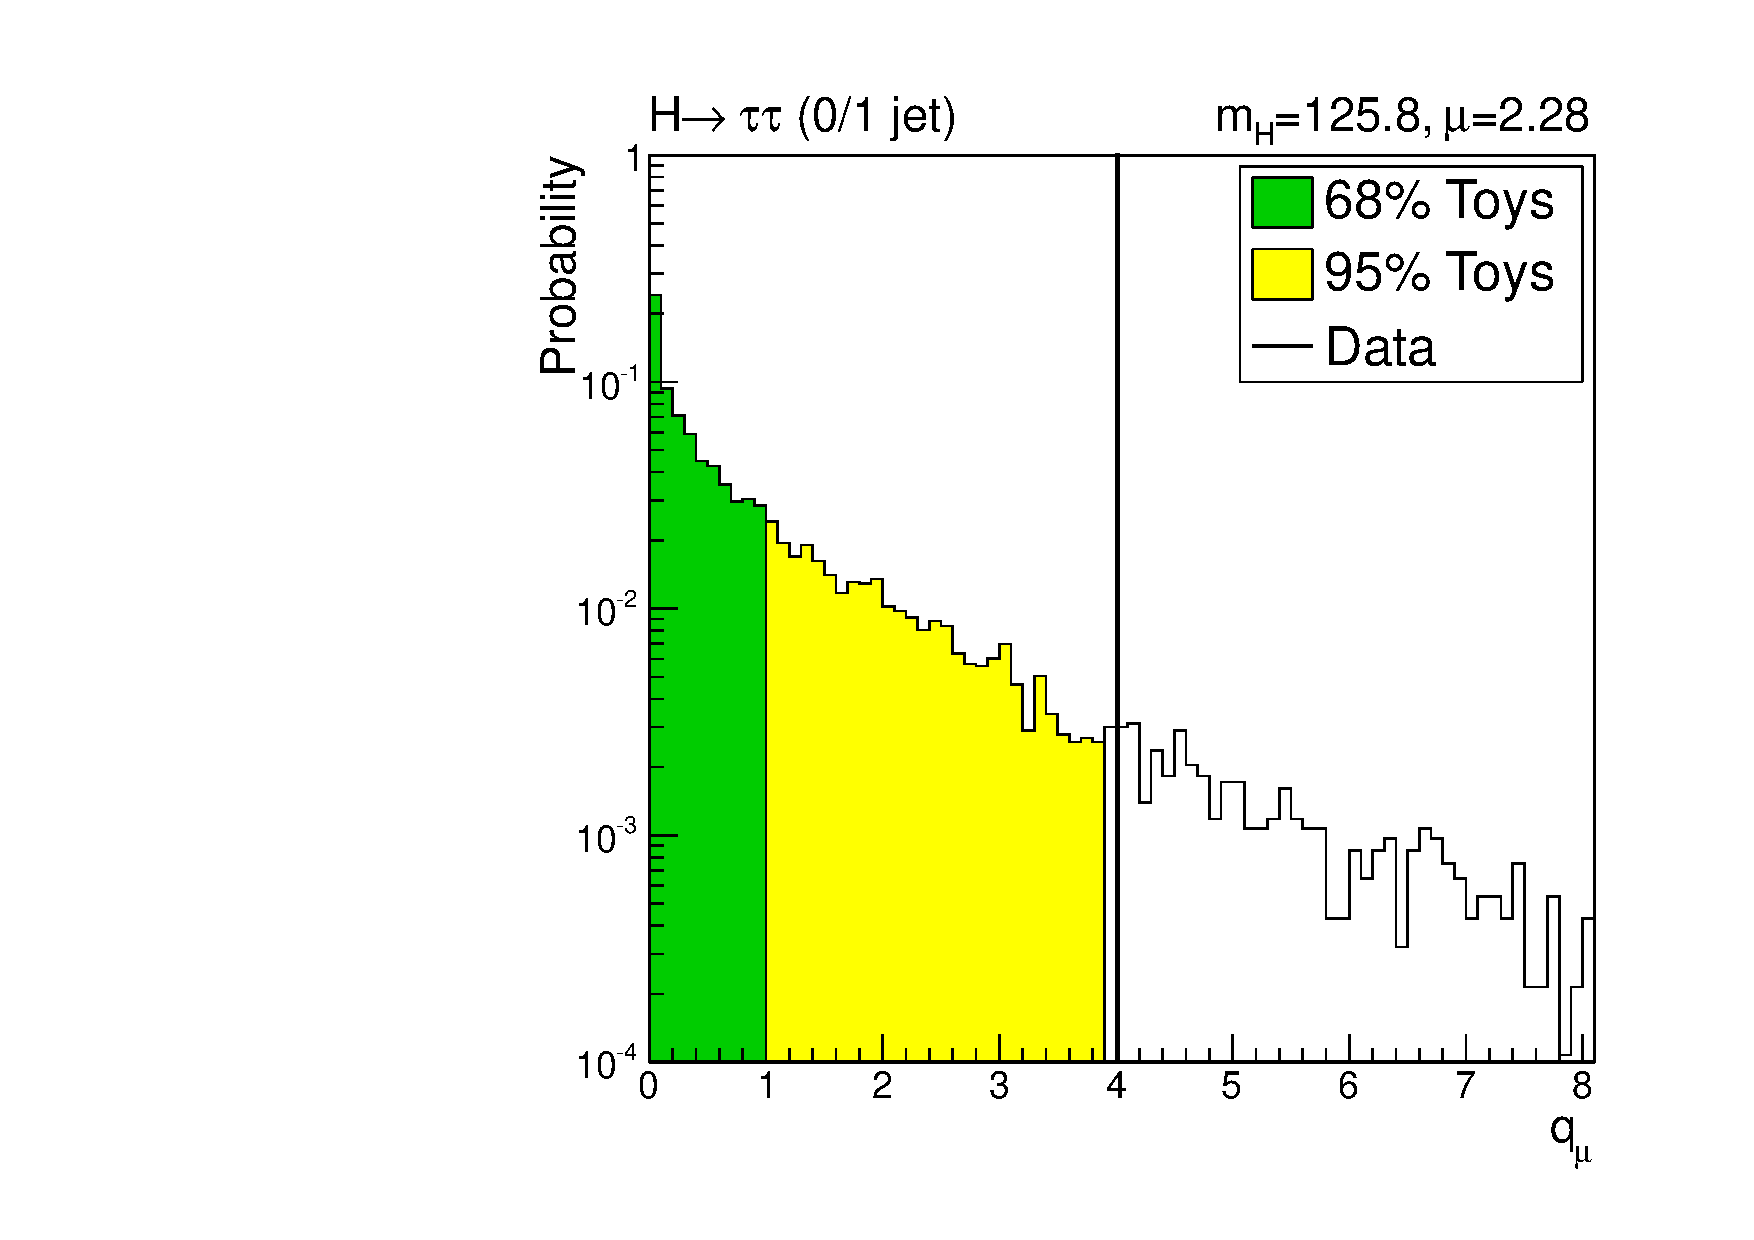
\includegraphics[width=.49\textwidth]{combinations/fceg_htt_2.pdf}
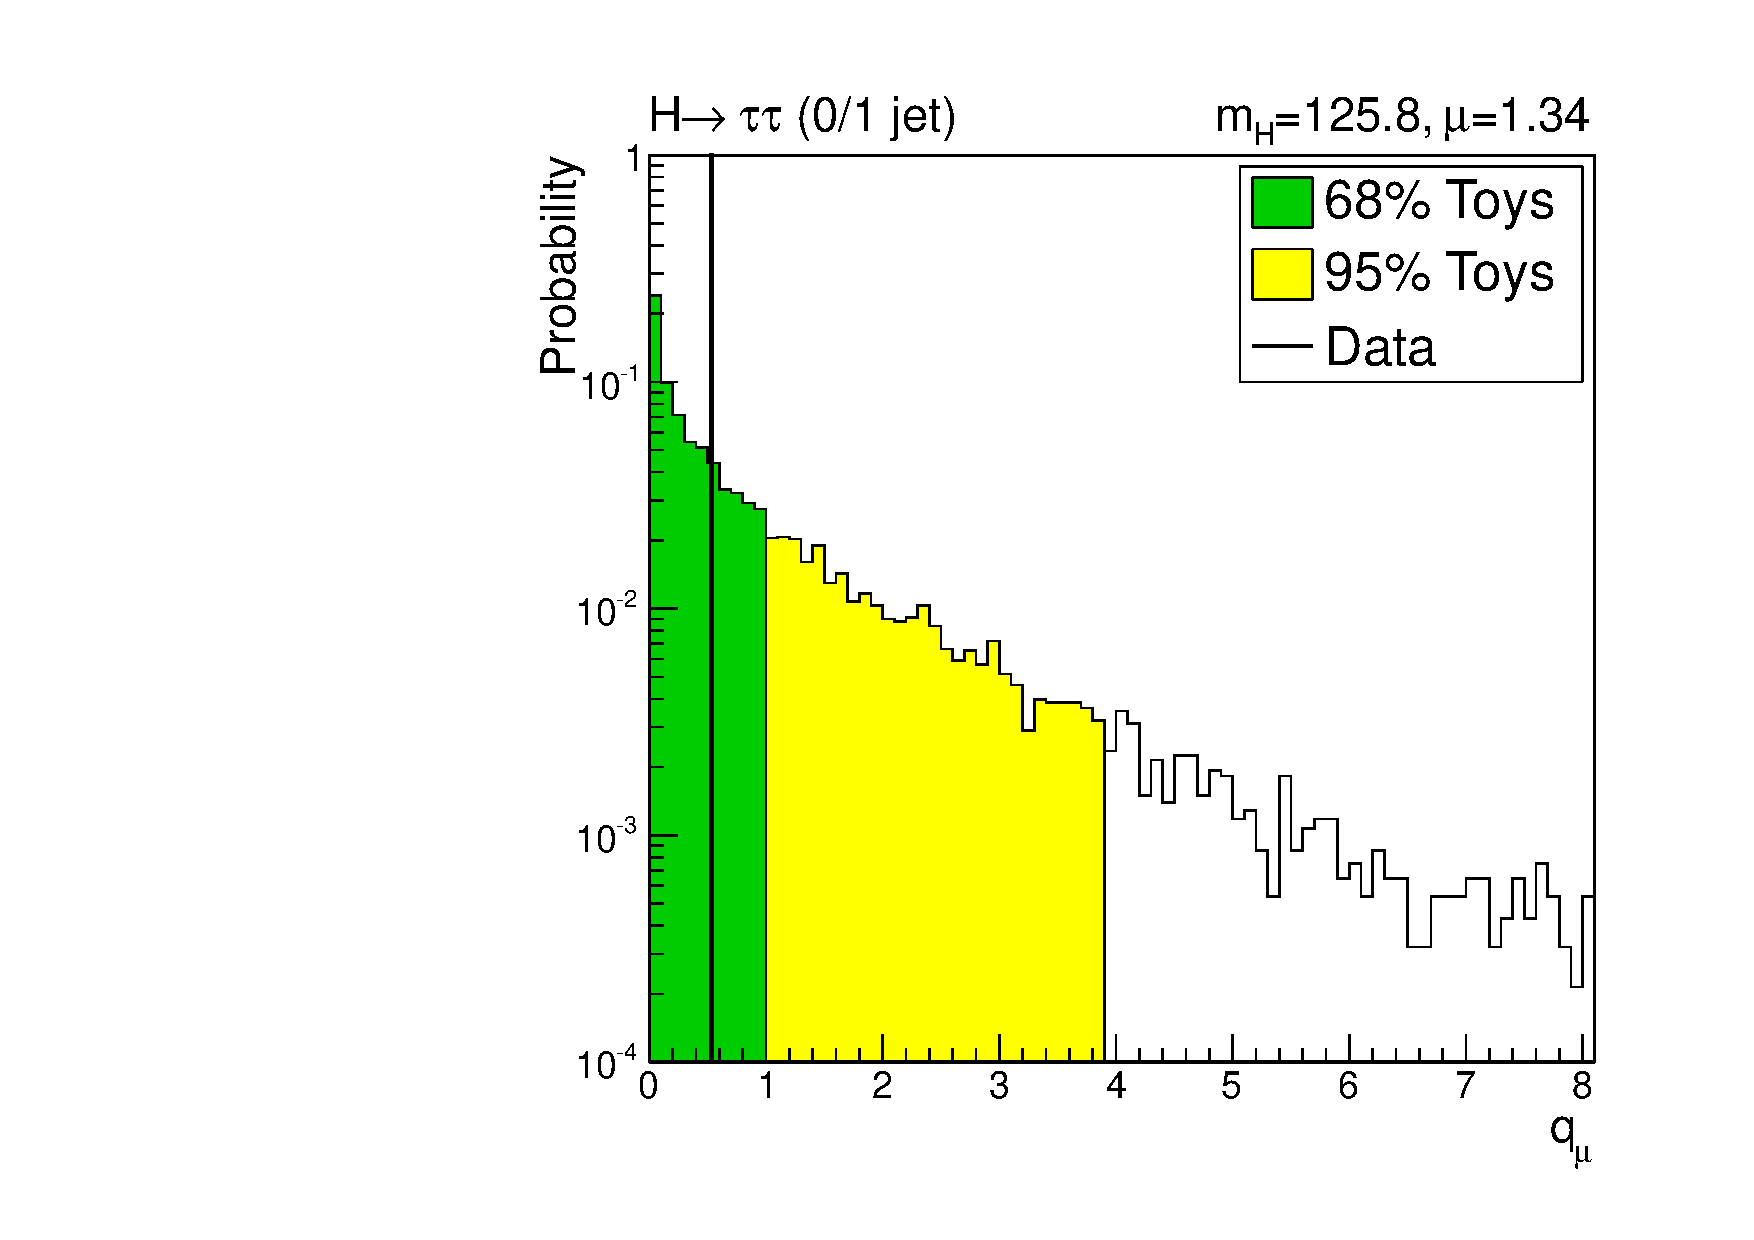
\includegraphics[width=.49\textwidth]{combinations/fceg_htt_1.pdf}
\caption{Distributions of the test statistic $q_{\mu}$ for the 0/1 jet bin 
of the $H\rightarrow \tau\tau$ analysis at the combined best fit mass, $m_{H} = 125.8$ GeV.
The green and yellow filled regions indicate the 68\% and 95\% quantiles of the 
distribution respectively. 
The left distribution is generated at $\mu=2.28$ 
which lies outside of the 68\% confidence interval
while the right distribution is generated at $\mu=1.34$ which lies inside the 
68\% confidence interval. The values of the test statistic obtained from the observed data, 
$q_{\mu}^{obs}$, are indicated by the solid vertical lines.}
\label{fig:fcegtoys}
\end{center}
\end{figure}
The 68\% confidence interval for $\mu$ is determined as the union of all values of $\mu$ for 
which $1-CL_{s+b}<0.68$.
Figure~\ref{fig:confcontour} shows the values of $1-CL_{s+b}$ for different values of 
$\mu$ in the 0/1 jet bin of the $\Htt$ analysis.
The vertical red line indicates $CL_{s+b}=0.68$ and the values at which the curve
crosses this line (indicated by the horizontal red lines) form the 68\% confidence 
interval for $\mu$.
\begin{figure}
\begin{center}
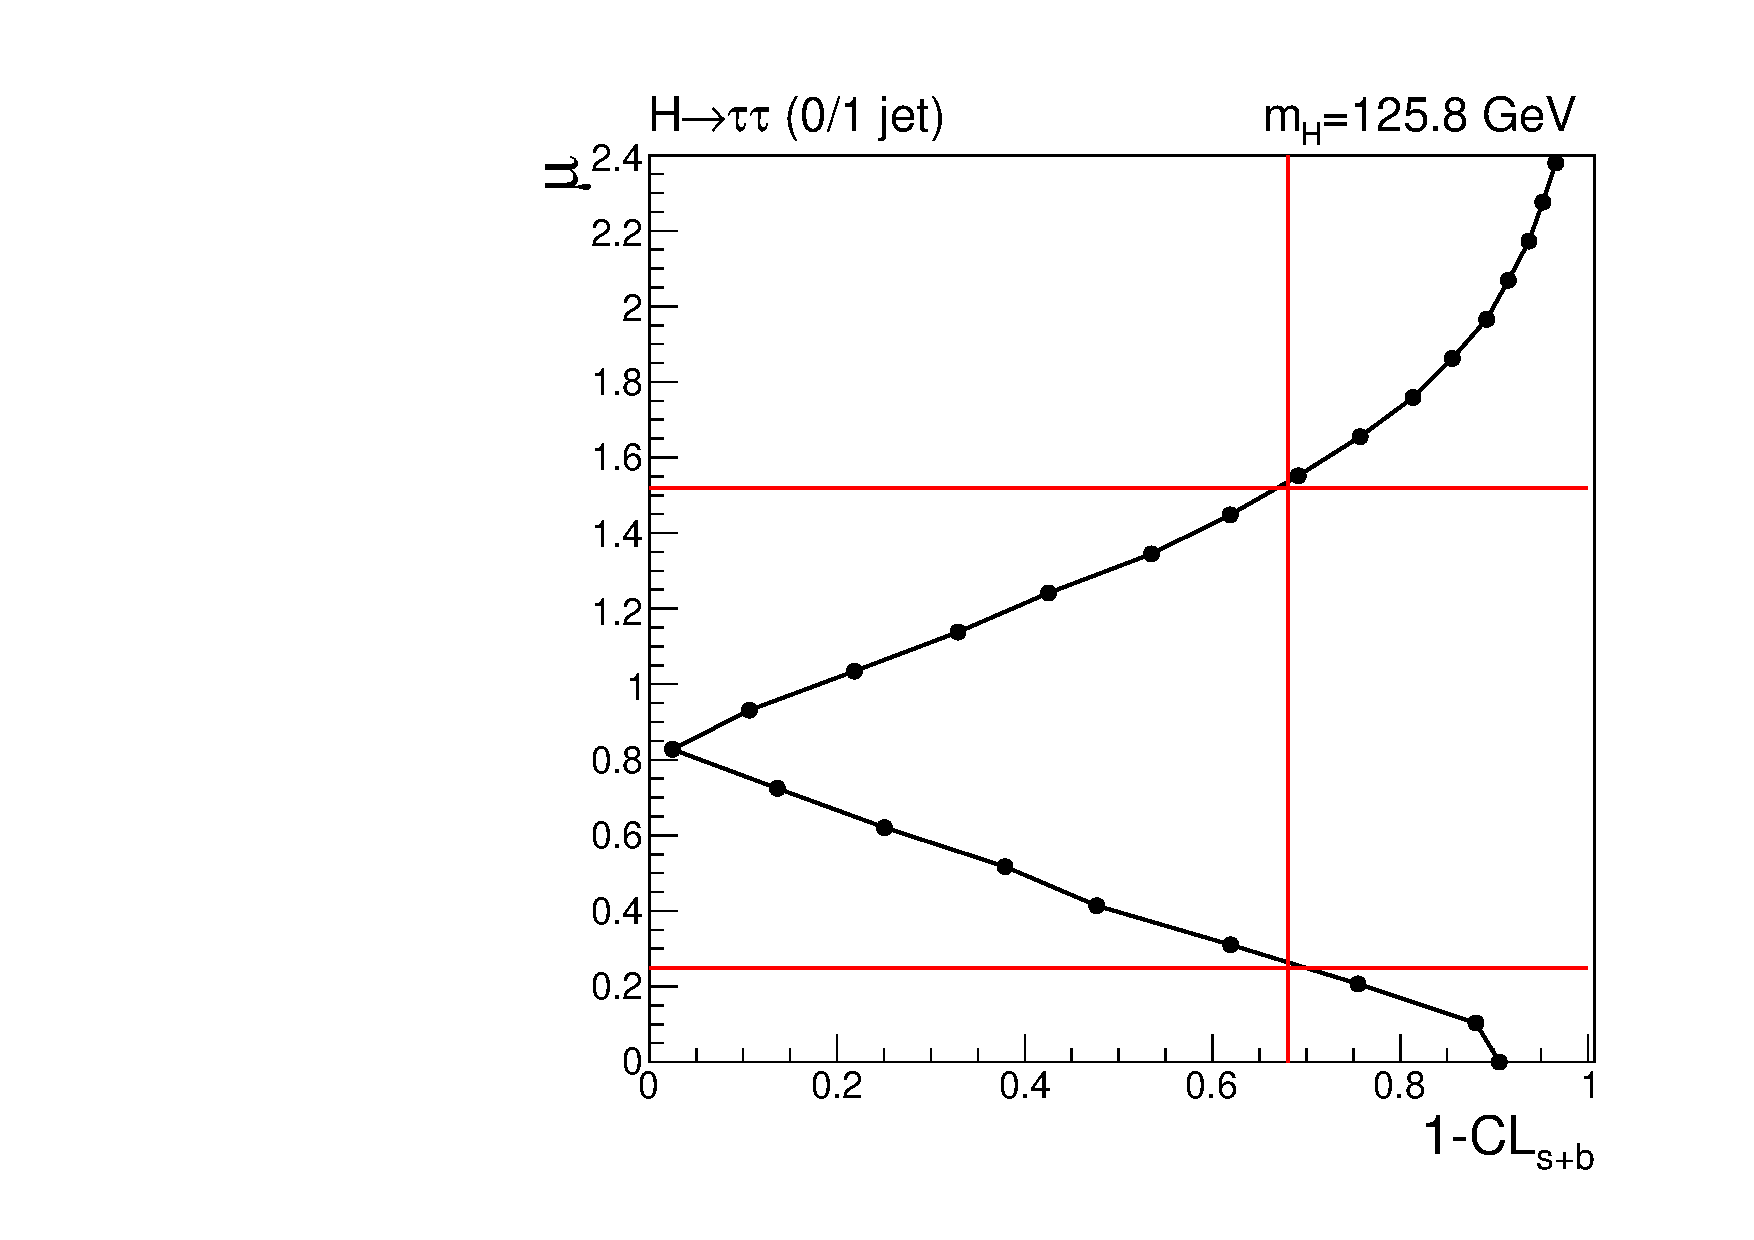
\includegraphics[width=.7\textwidth]{combinations/confcurve_htt.pdf}
\caption{Confidence level evaluation curve for the $\Htt$ analysis in the (0/1) jet bin. 
At each point, pseudo-data are generated with signal injected at the given value of $\mu$
and its confidence level (CL) calculated.
Linear interpolation between the generated points is used to determine the 68\% confidence 
interval; the two values of $\mu$ (horizontal lines) which cross the curve at $1-CL_{s+b}=0.68$
(vertical red line).}
\label{fig:confcontour}
\end{center}
\end{figure}
The procedure is easily extended to a higher number of dimensions
by exchanging the test-statistic for $q_{\boldmu}$, given in Equation~\ref{eqn:llrNd}.
Pseudo-datasets are generated and fit as before and the union of points for which
$1-CL_{s+b}<0.68$ defines a confidence-contour in an $n$-dimensional parameter space.


\subsection{Combined Mass Measurement}
The mass of the Higgs boson is a free parameter in the context of the 
Standard Model. The high resolution channels, 
$\Hgg$ and $\Hzz \rightarrow 4l$, 
provide the strongest constraint on the mass of the new particle as the signal
is visible as a narrow peak in the invariant mass of its decay products.
To measure the mass, $m_{X}$, of the particle in a model-independent way,
the signal strengths for the $gg\rightarrow \Hgg$, $qq\rightarrow \Hgg$
and $\Hzz\rightarrow 4l$ processes are assumed to be independent and thus are treated as 
nuisance parameters in the likelihood. Each of the signals in these channels
are assumed to be due to the presence of a single state with mass $m_{X}$.
Figure~\ref{fig:mass} (left) shows the value of the test-statistic 
$q_{m_{X}}$ for the $\Hgg$, $\Hzz$ channels and their combination near the
best fit points. From the combination, the mass is determined to be $m_{X}=125.8 \pm 0.5$ GeV.
The 68\% confidence interval is determined
from the values of $m_{X}$ at which the curve crosses the horizontal red line at 1.
Large background fluctuations in the $\Hgg$ channel can result in
large variations of the measured mass when the signal is small.  
Conversely, the kinematic constraints on the $4l$ system cause a large variation in
the branching ratio of $\Hzz \rightarrow 4l$, and hence the expected signal yield, 
as a function of $\mh$.
Figure~\ref{fig:mass} (right) shows the two-dimensional 68\% confidence intervals
in $m_{X}$ and $\xs$ for the $\Hzz\rightarrow 4l$, $\Hgg$ and their combination.
For this combination, the ratio signal strengths between the two channels is
kept fixed to the SM expectation; only the overall signal strength is left as a 
free parameter.  The best fit value of $m_{X}$ is consistent with the 
value determined in the one-dimensional case. 
The best fit value for the combined signal strength relative to the 
Standard Model is $0.88\pm0.21$ for a mass of 125.8 GeV.

\begin{figure}
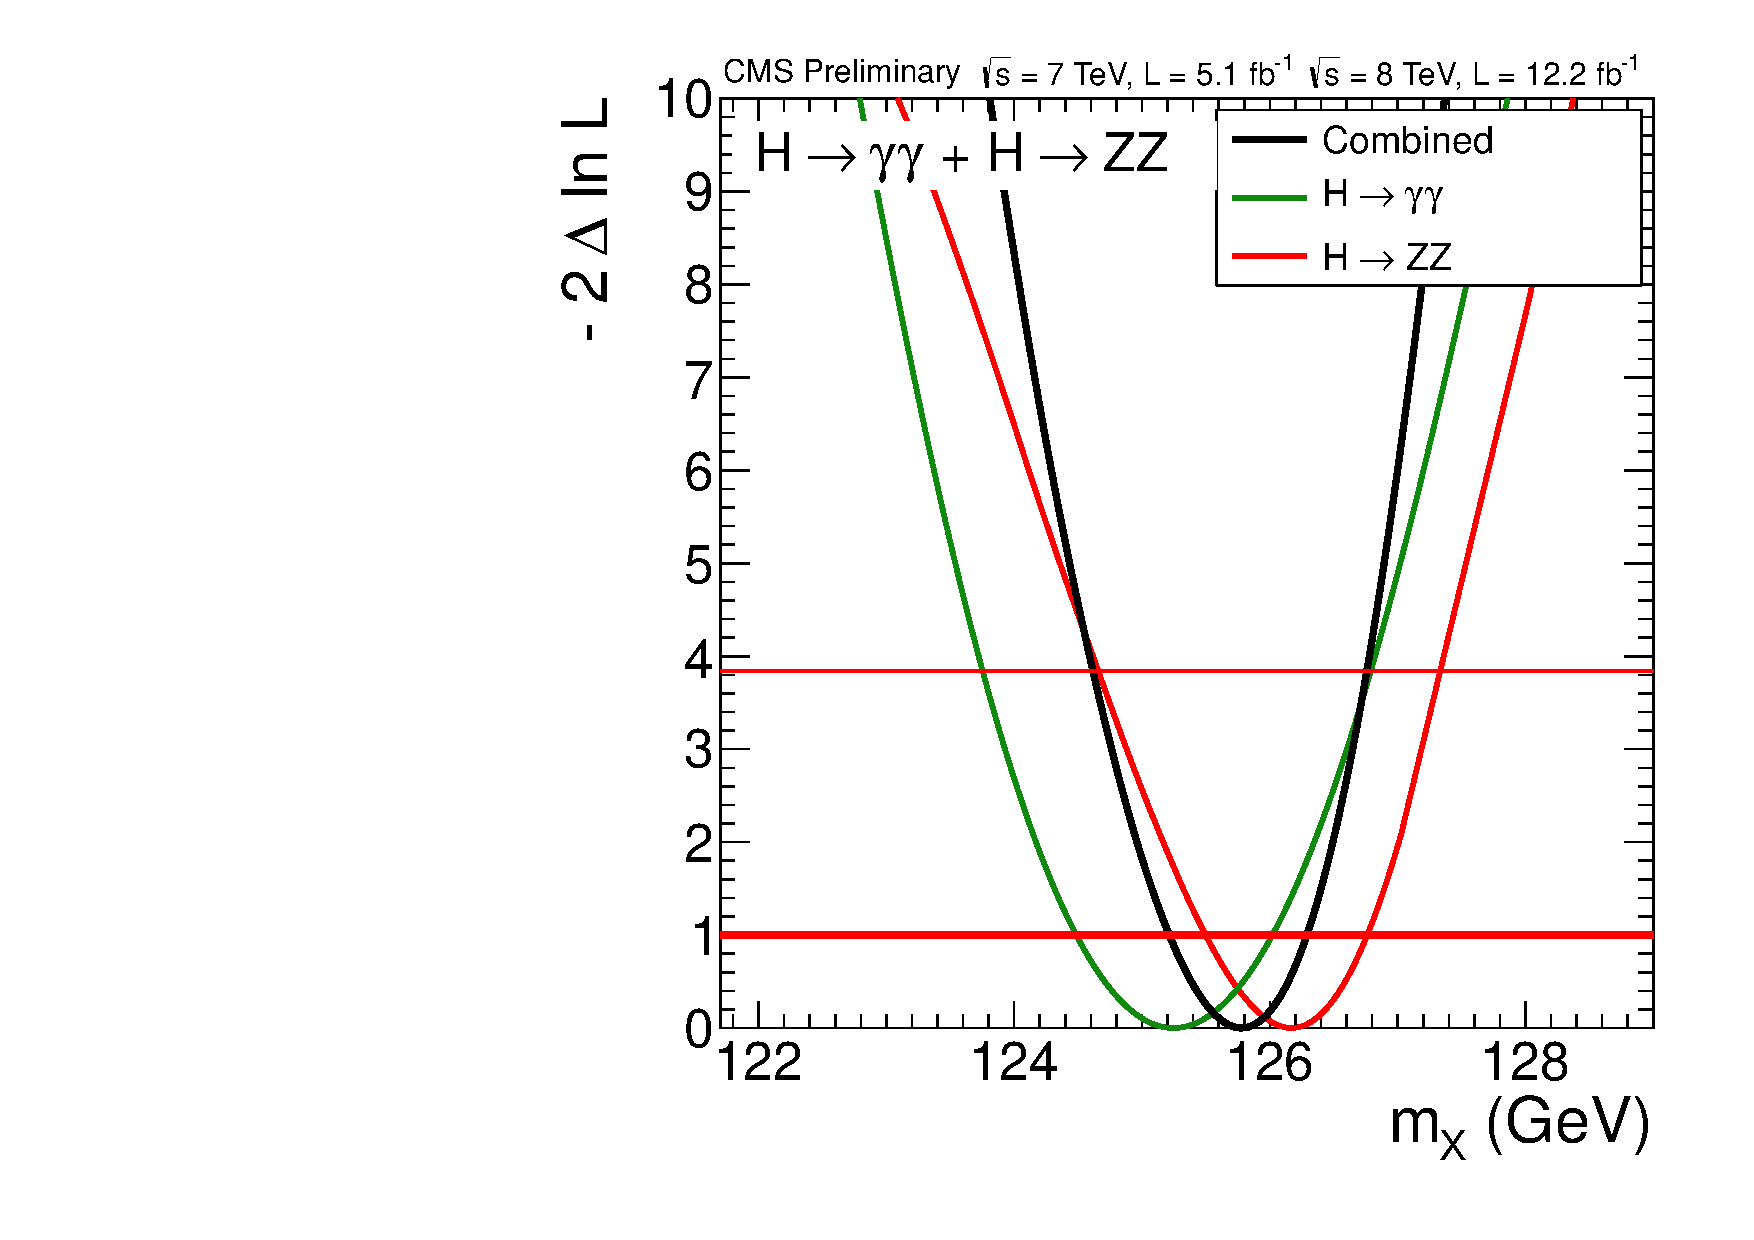
\includegraphics[width=0.49\textwidth]{combinations/Figure_007-b.pdf}
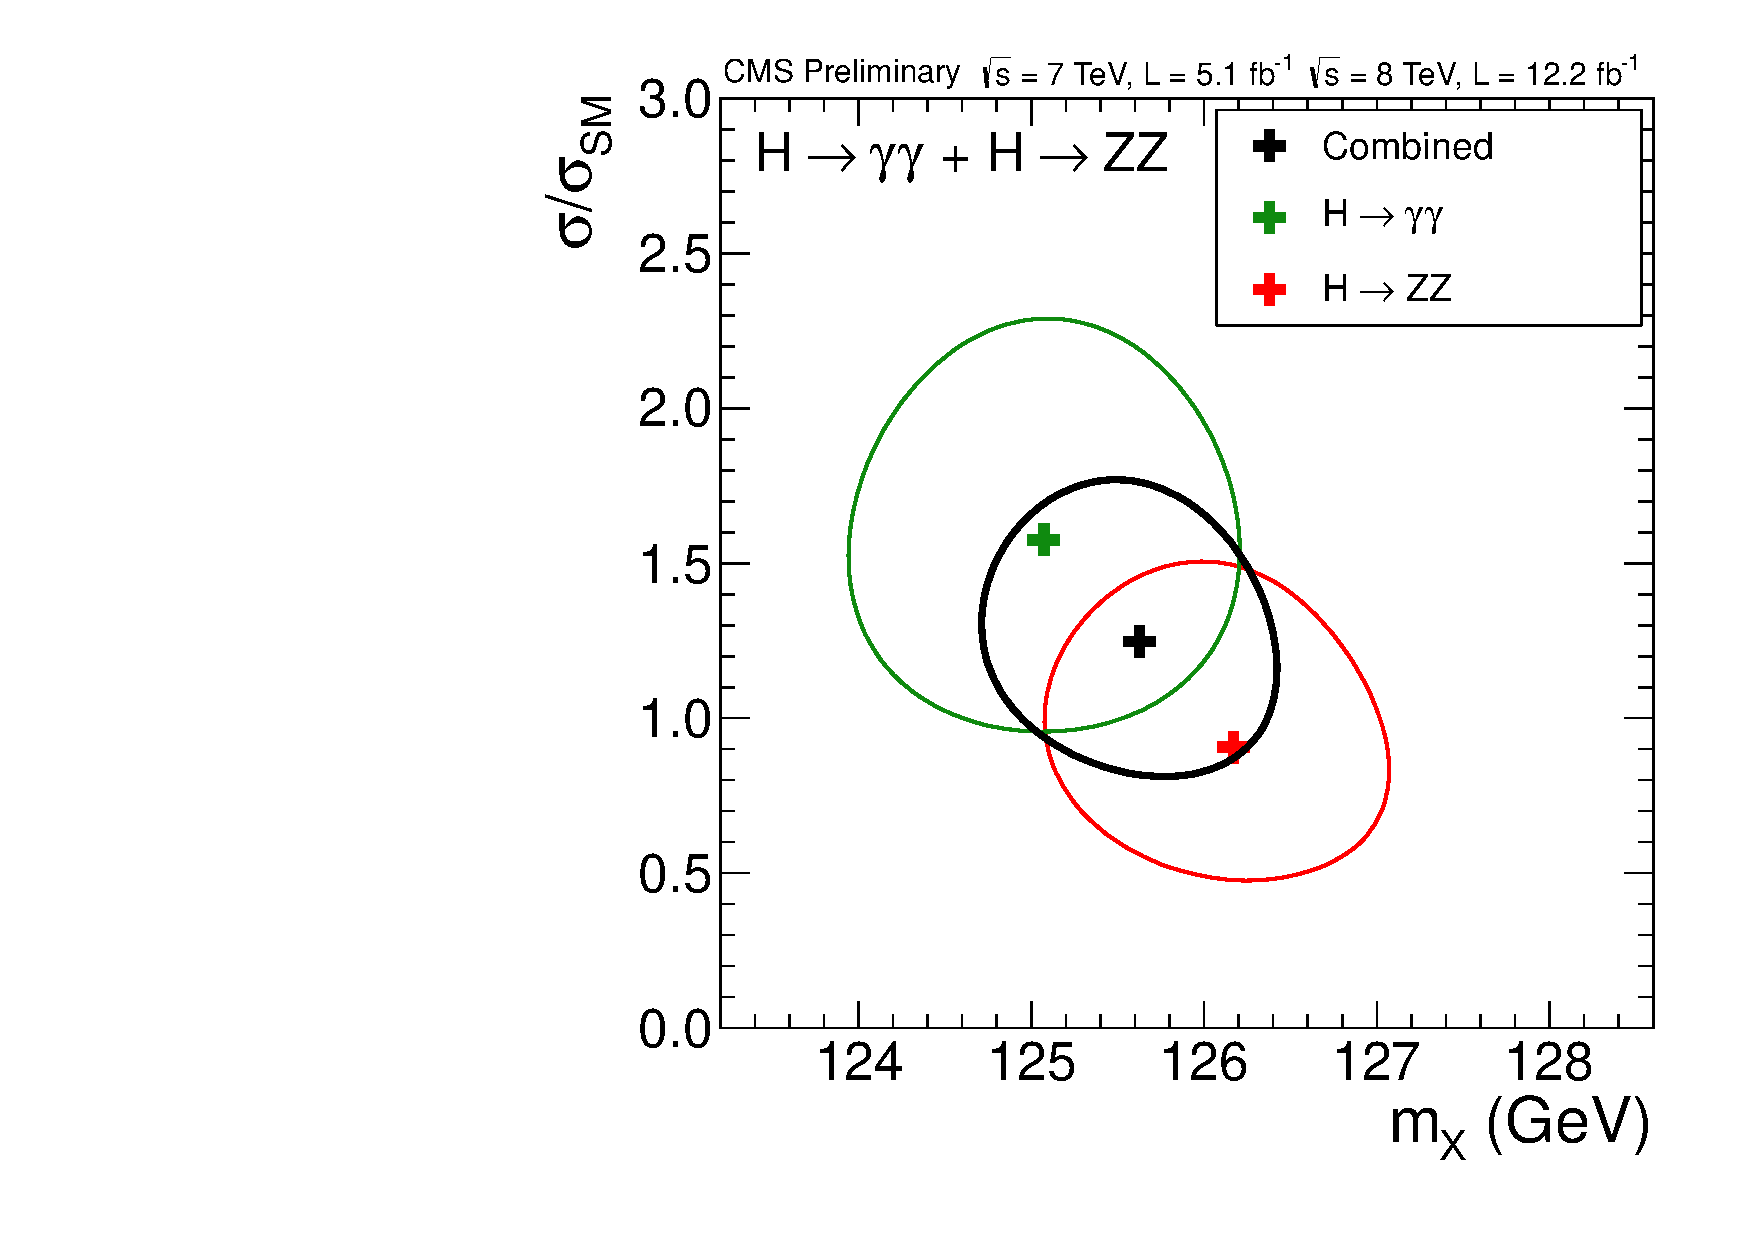
\includegraphics[width=0.49\textwidth]{combinations/Figure_007-a.pdf}
\caption{ Left: One-dimensional scan of $q_{m_{x}}$ for the $\Hgg$,
$\Hzz$ channels and their combination. For the combination, the relative
signal strengths between the channels are allowed to float. The 68\%
and 95\% confidence intervals for $m_{X}$ are determined as the values at
which the curves cross the horizontal red lines. Right: 68\% confidence
contours in $m_{X}$ and $\xs$ for the $\Hgg$ and $\Hzz$ channels and their
combination. For this combination, the relative signal strengths of the 
channels are kept fixed to the SM expectation.}
\label{fig:mass}
\end{figure}
\subsection{Compatibility with the Standard Model}
The Standard Model makes very precise predictions for the coupling of the Higgs 
boson to all of the known fundamental particles. These couplings directly influence 
the various rates of production and decay of the Higgs boson. 
Precise measurements of these rates 
in the combined search channels provide information on the couplings. 
Significant deviations from the values predicted by the SM 
would indicate the presence of new physics.

\subsubsection{Channel Compatibility}
When determining the preferred value of $\mu$ in the combined data, 
the ratios of decay rates to each contributing channel relative 
to that predicted by the SM are kept constant. 
By relaxing this constraint, the compatibility of the new state 
with the SM Higgs boson can be studied on a per-decay/per-production level. 
Due to the limited amount of data collected at CMS, 
some of the channels and sub-channels entering the combination
have a negative value for the best fit signal strength ($\mu=\xs$).
In order to avoid quoting unphysical values in each channel, the Feldman-Cousins
procedure is used to determine 68\% confidence intervals for $\xs$ separately in the different
channels/sub-channels entering the combination. 
Figure~\ref{fig:fc1d} (left) shows the 68\% confidence intervals on $\xs$ for the sub-channels 
included in the combination obtained from the HCP dataset. The results are compared with the intervals determined
directly from a scan of $\qmu$, as shown in the same figure (right). The two methods are found
to be in good agreement. The intervals are extracted for a Higgs boson 
mass $m_{H}=125.8$ GeV (the overall best fit mass of the new state obtained from the
same dataset). The 68\% confidence interval on $\xs$ for the full combination is indicated
by the green band. With the exception of the dijet (VBF) tagged channel in the 
$\Hgg$ analysis, all of the intervals contain the value $\mu=1$ which is the expected value for 
a SM Higgs boson. 
\begin{figure}
\begin{center}
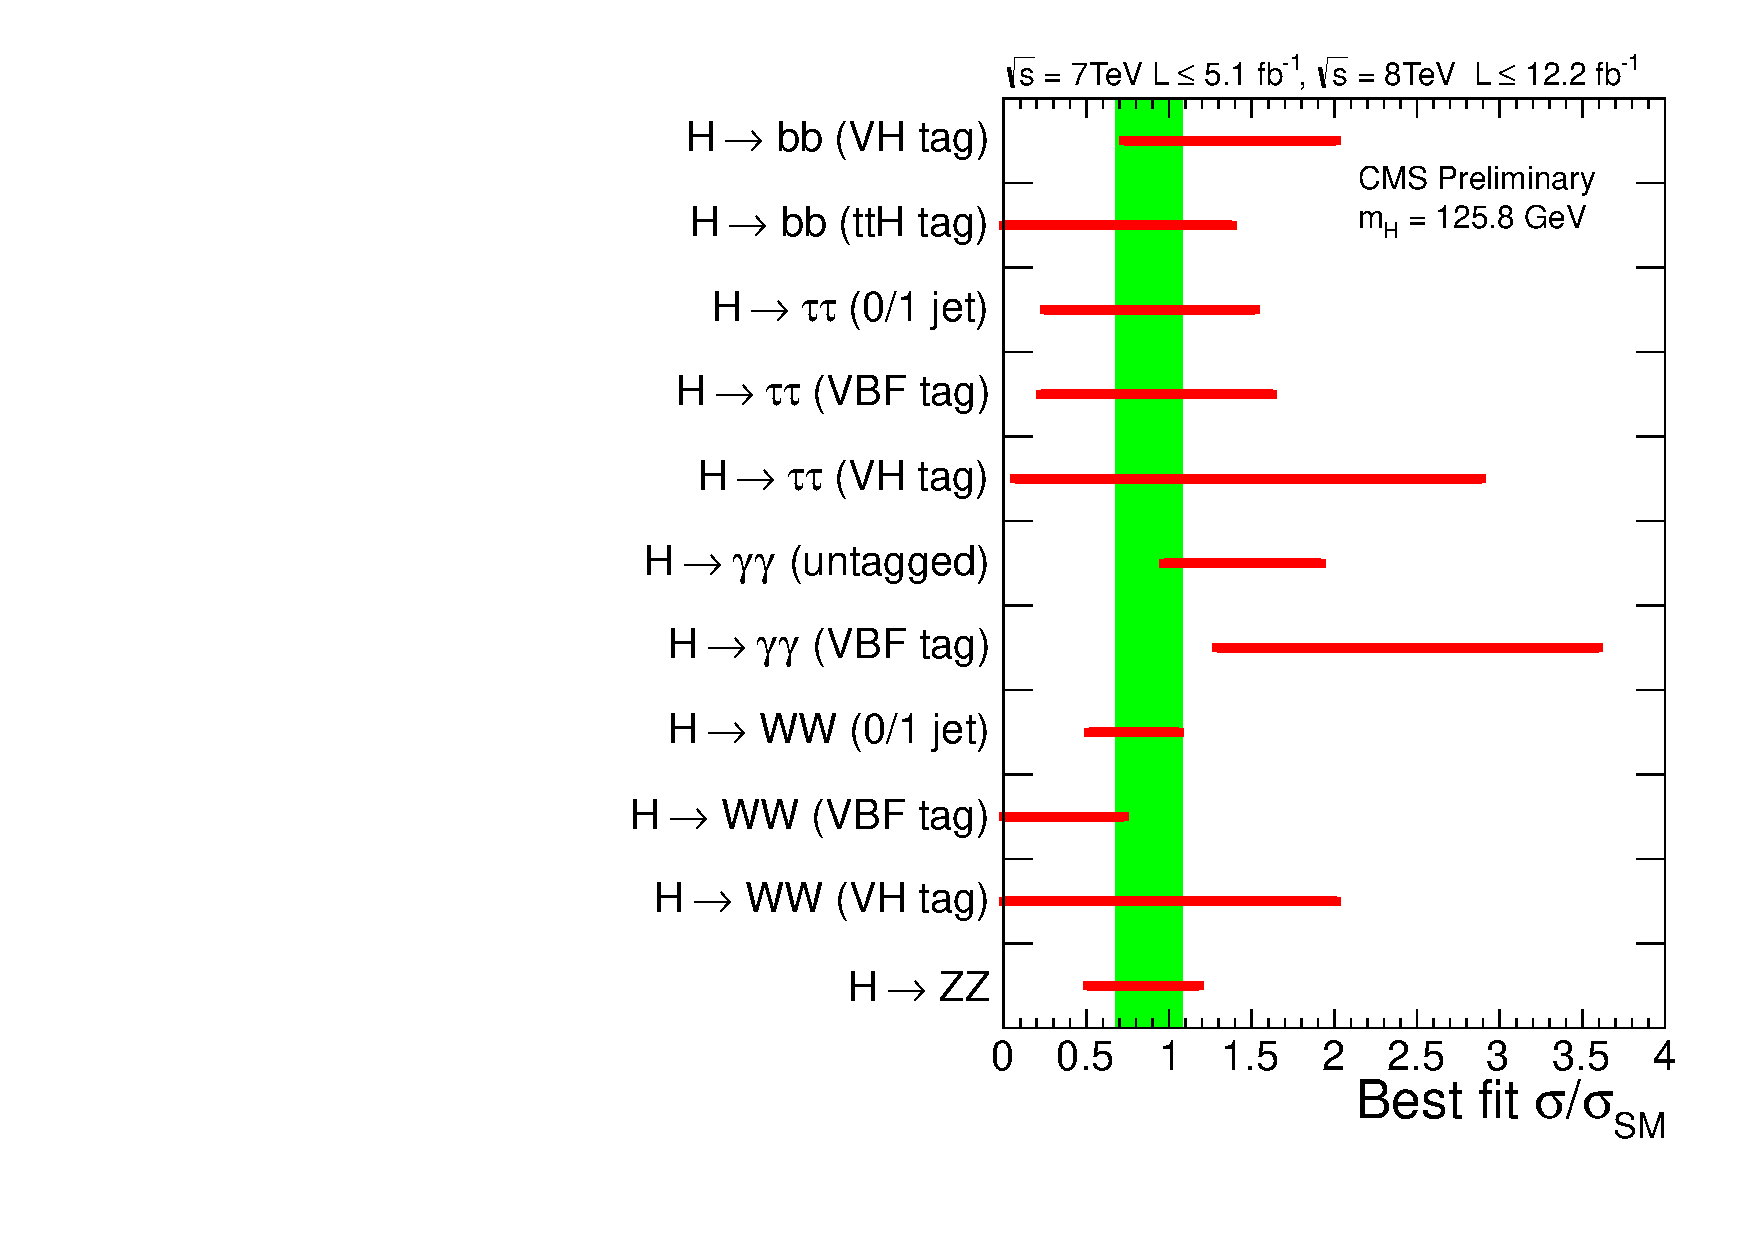
\includegraphics[width=.49\textwidth]{combinations/sqr_fc_ccc.pdf}
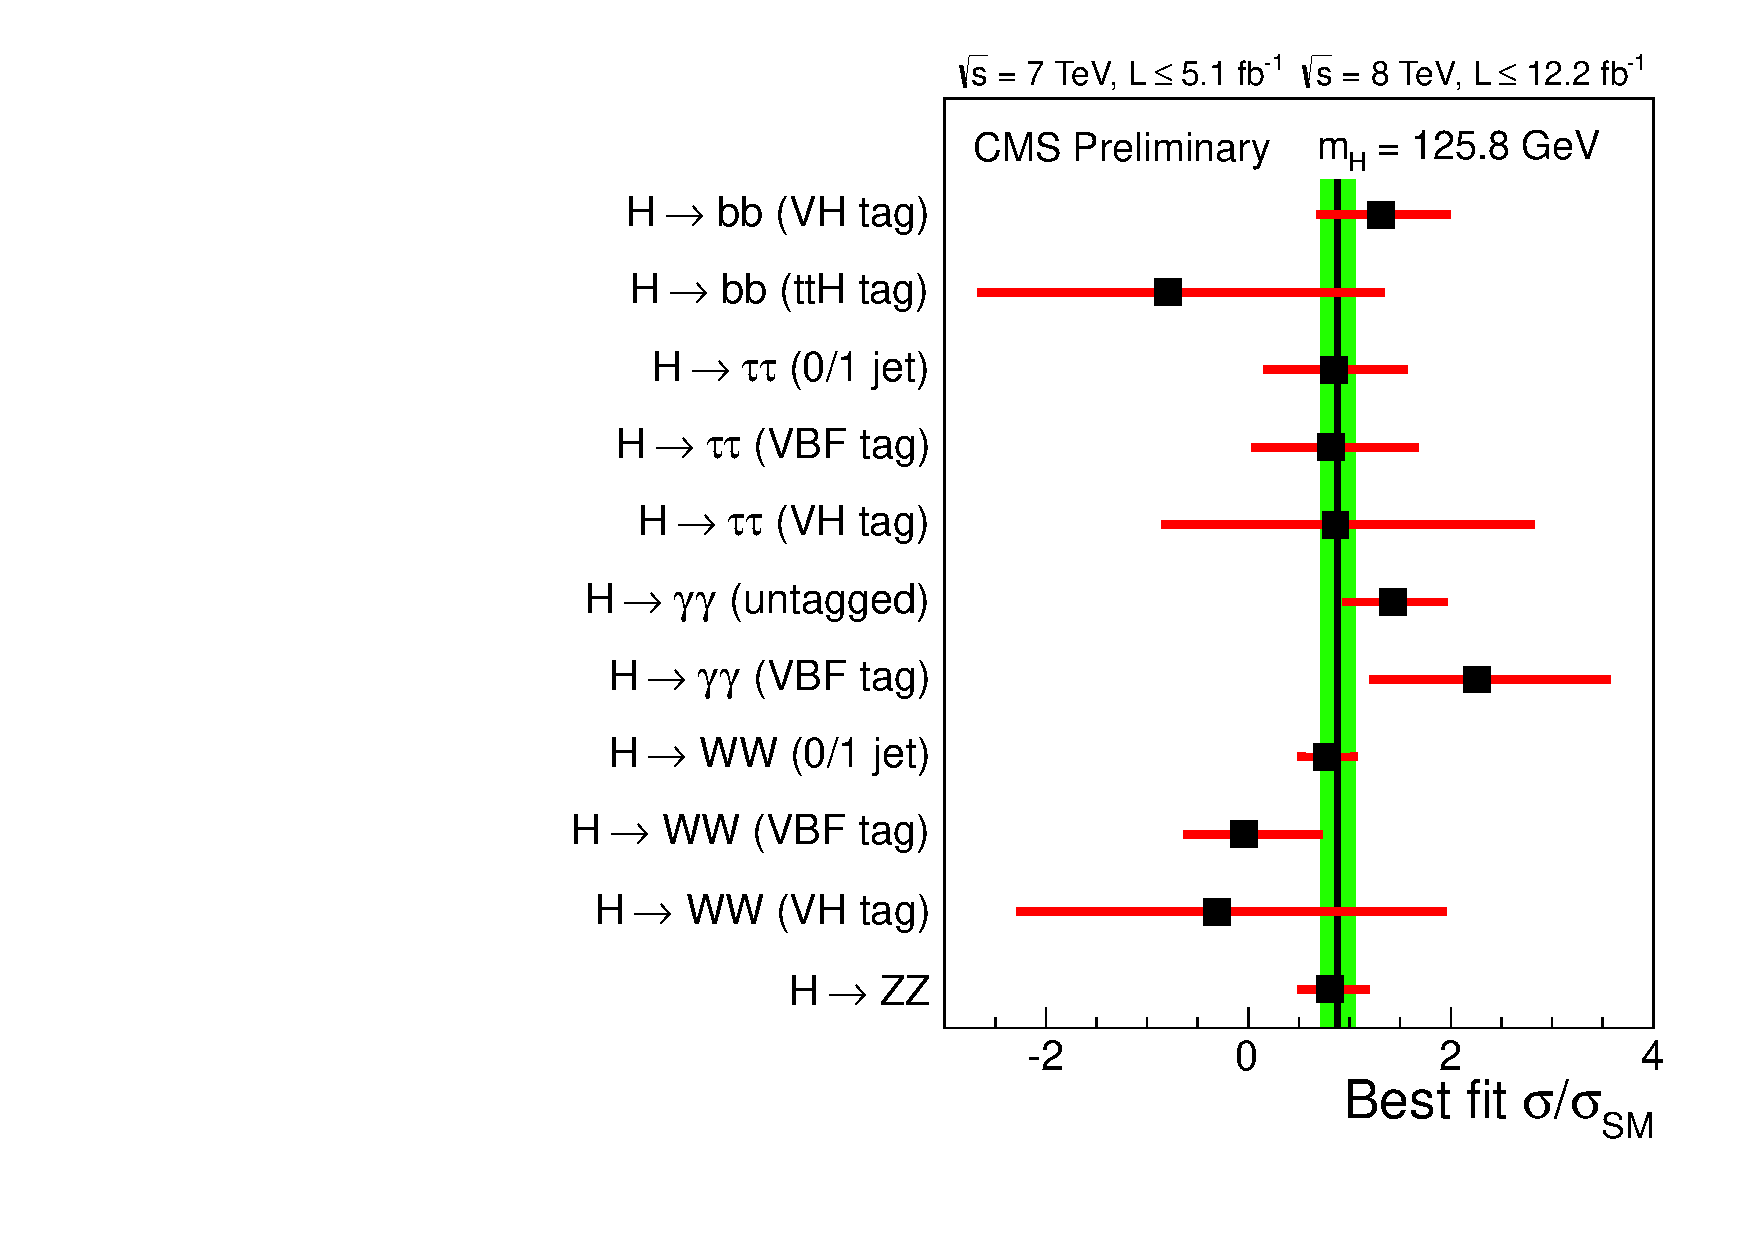
\includegraphics[width=.49\textwidth]{combinations/sqr_mlz_ccc_mH125.pdf}
\caption{68\% confidence intervals for $\mu=\xs$ for individual 
channels or combination of sub-channels determined using the Feldman-Cousins procedure (left) 
and by scanning the likelihood (right). The value of $\xs$ denotes
the production cross-section times the relevant branching fraction for a given 
channel, relative to the SM. The green band indicates the 68\% confidence interval
on $\xs$ for all channels combined. The intervals are determined at the best fit 
mass, $m_{H}=125.8$ GeV.}
\end{center}
\label{fig:fc1d}
\end{figure}

Several of the analyses which are combined in the search for the Higgs boson use  
selections (tags) which are specifically designed 
to enhance the sensitivity to particular Higgs boson 
production topologies. The $\Hww$, $\Htt$ and $\Hgg$ analyses all include
dijet (or VBF tagged) categories which are designed predominantly to select events 
produced via vector-boson fusion ($qqH$). 
Additional sensitivity is gained in the $\Hww$, $\Htt$ and $\Hbb$ channels by 
looking for additional leptons or $E_{T}$ in association with production of 
a vector boson ($VH$). The production rates associated 
to couplings with top-quarks ($ggH$ and $ttH$) and vector bosons ($qqH$ and $VH$) 
are determined by removing the requirement that the relative production 
cross-sections $\muggh$ and $\muqqh$ are equal.
The compatibility of the rates observed in data with respect to those
predicted by the Standard Model can be tested using the Feldman-Cousins
procedure or scanning the test-statistic $q_{\boldmu}$. The relative branching ratios to each of the five observable final states
are left unconstrained.
Figure~\ref{fig:fc2d} shows the 68\% confidence contours for each
of the five decay processes using the two methods. Good agreement is found when comparing the two methods. 
With the exception of the $\Hzz$ analysis, the
explicit exploitation of the different production modes leads to 
elliptical contours. The SM point $(1,1)$, indicated by the yellow diamond, 
is contained within the 68\% confidence contours from each decay channel with the 
exception of $\Hgg$.  

\begin{figure}
\begin{center}
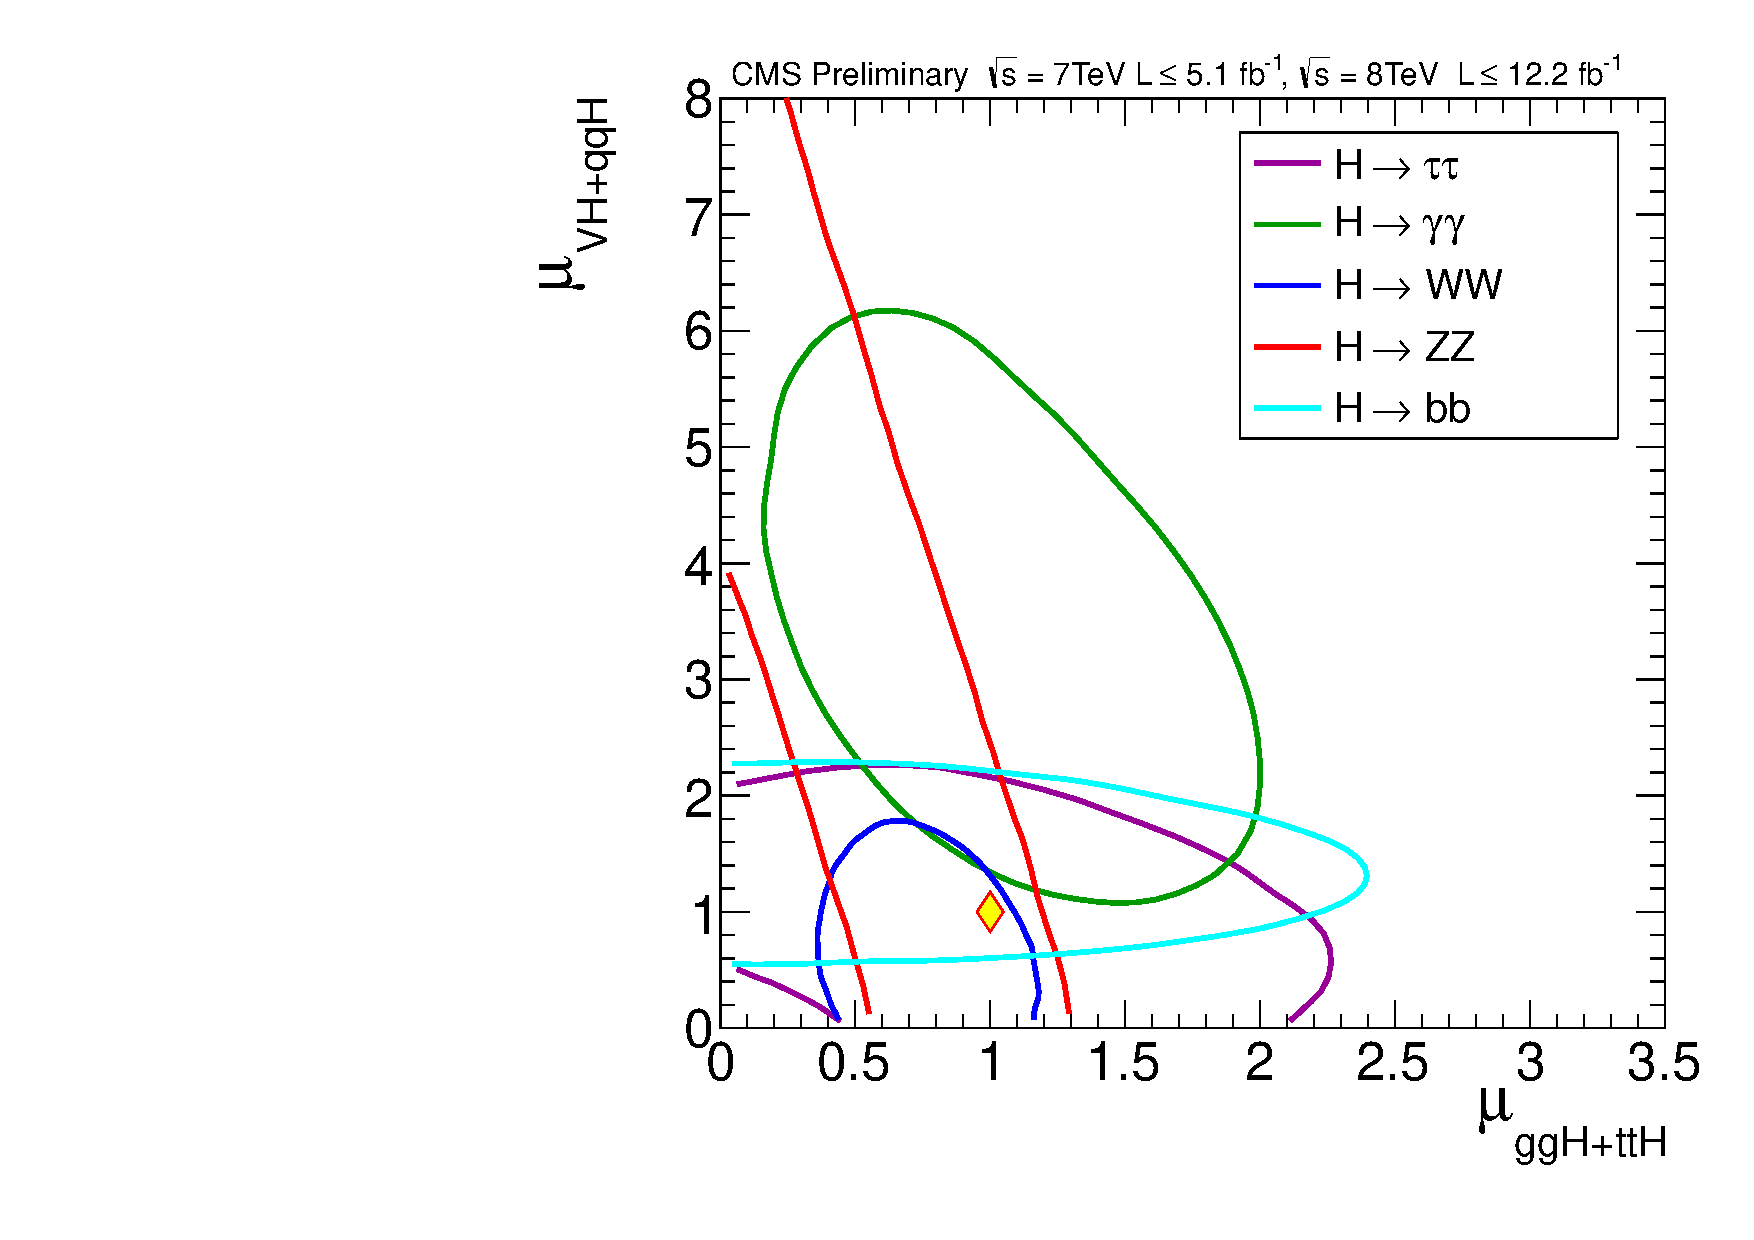
\includegraphics[width=.49\textwidth]{combinations/sqr_rvrf_fc_2d.pdf}
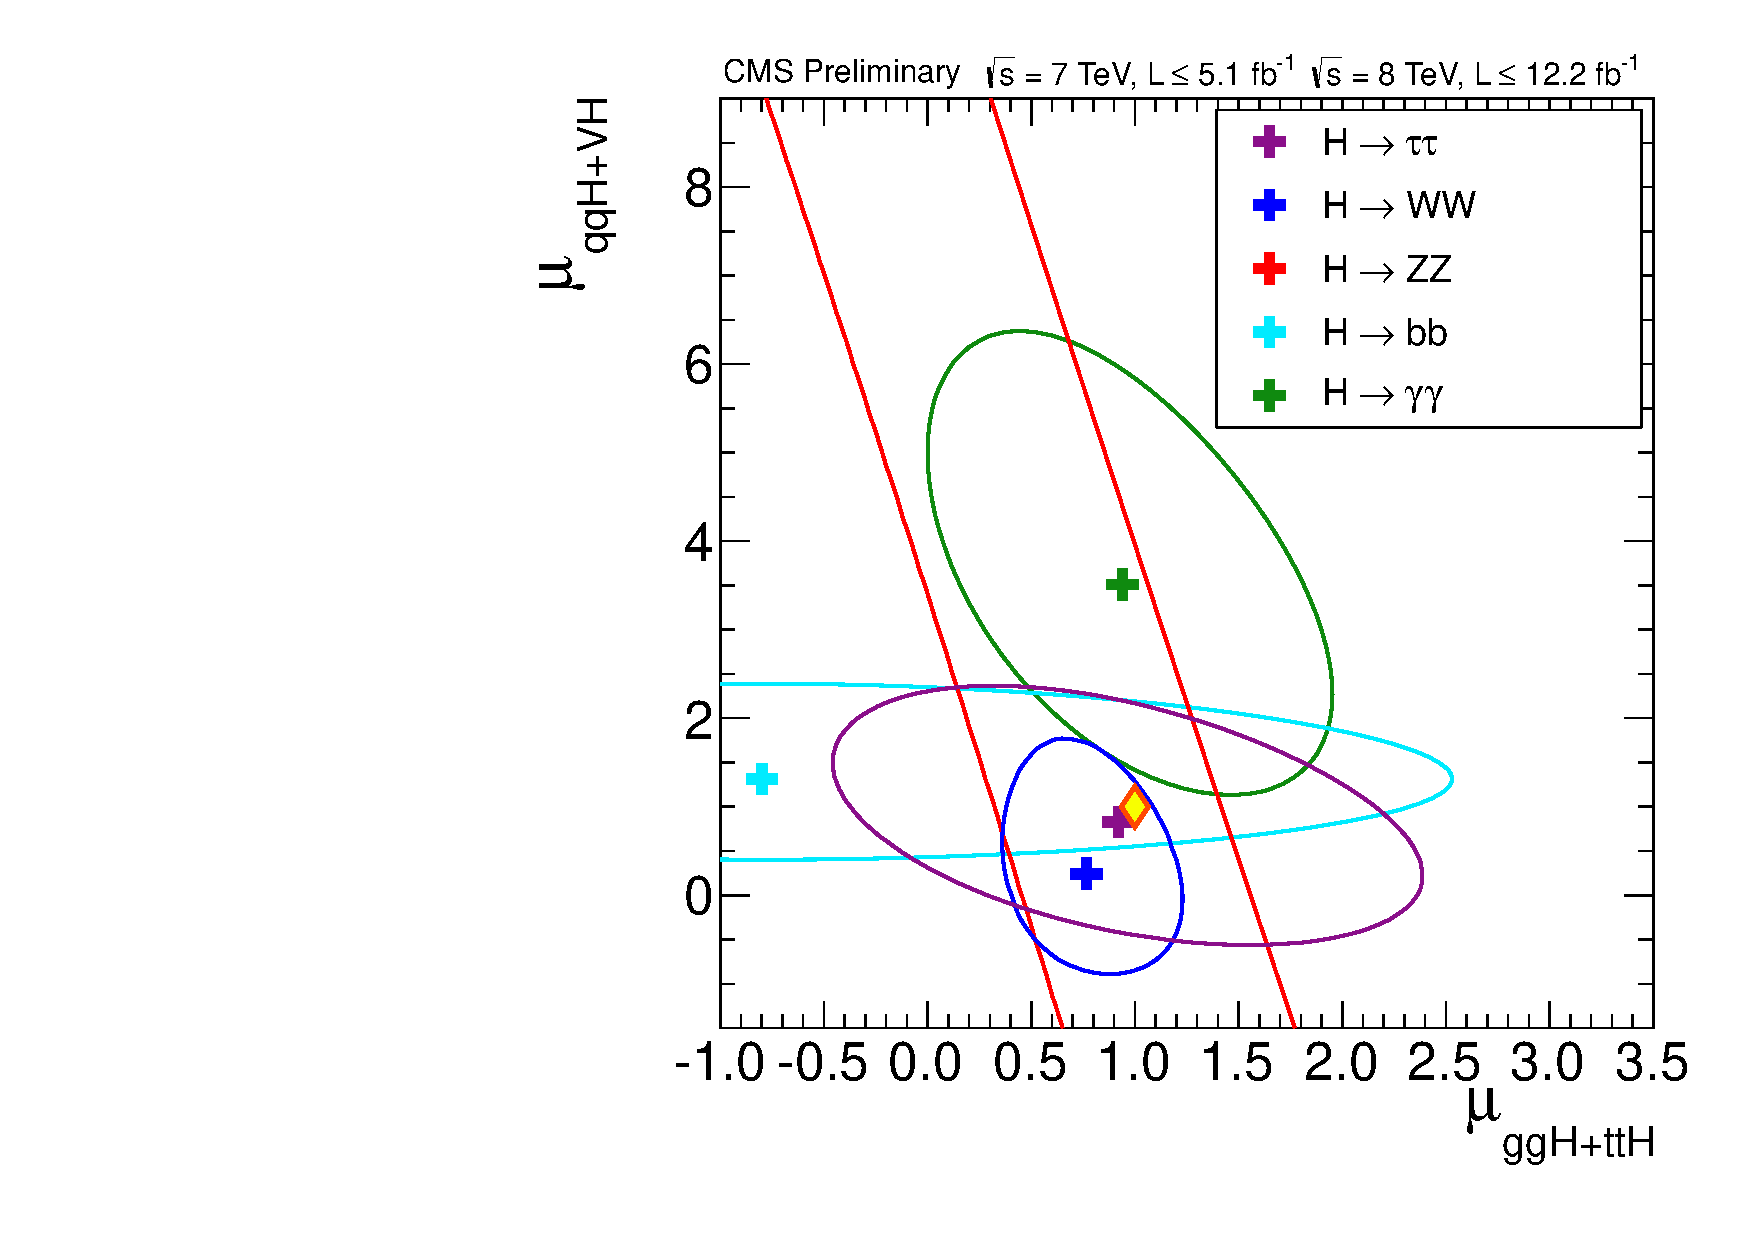
\includegraphics[width=.49\textwidth]{combinations/sqr_rvrf_scan_2d_all_68.pdf}
\caption{68\% confidence contours for the production cross-section in 
$ggH$ and $ttH$ modes ($\muggh$), and $VH$ and $qqH$ modes ($\muqqh$), 
relative to the SM determined using the Feldman-Cousins procedure (left) and 
by scanning the likelihood (right). 
Each colour indicates the result by combining all sub-channels in a particular
decay mode. The crosses indicate the best fit values of the two parameters.
The yellow diamond at $(1,1)$ indicates the SM values. 
The contours are determined at the best fit mass, $m_{H}=125.8$ GeV.}
\end{center}
\label{fig:fc2d}
\end{figure}


% This section might not make it into the final draft, bit too out there?
\subsubsection{Coupling Measurements}
\label{sec:coupling}

The compatibility of the couplings of the new particle with the SM cannot be directly ascertained 
in the experimental data. In order to extract the relevant information, the rates of production and decay in the various
channels must be interpreted in terms of the underlying couplings to the SM particles.
For the purposes of evaluating the compatibility in the couplings, the following simplifications
are made:
\begin{itemize}
\item Signals observed in each of the different search channels originate from a single
resonance near 125 GeV.
\item The natural width of the resonance is small enough to be neglected such that the 
cross-section of the signal in each channel can be expressed as
\begin{equation}
(\sigma \cdot BR)(ii\rightarrow H\rightarrow ff) 
	= \frac{\displaystyle \sigma_{ii}\Gamma_{ff}}{\displaystyle \Gamma},
\end{equation}
where $\sigma_{ii}$ is the production cross-section through the initial state $ii$, 
$\Gamma_{ff}$ is the partial decay width to the final state $ff$ and $\Gamma$ is the
total width. 
\item Only modifications of the absolute values of the coupling strengths are allowed. 
The structure of the couplings is fixed to the SM, in particular this means the 
new state is assumed to be a CP-even scalar.
\end{itemize}
In general, no specific assumptions are made on any additional states of new physics
which could influence the phenomenology of the 125 GeV state.
A number of frameworks to investigate the coupling structure of the new particle
are used at CMS~\citep{couplingsint}. The simplest of these is an unfolding of the production cross-section
modifiers $\mu_{ttH+ggH},~\mu_{VH+qqH}$ by expressing them as functions of the couplings 
to fermions $\kf$ and vector bosons $\kv$ and is described here as an example. 
The decay rates to each channel are also expressed as functions of these parameters such that the overall 
yield in each channel relative to the SM expectation is parameterized.
The ratio of the total width to that predicted by the SM is denoted $\kappa_{H} =\Gamma/\Gamma_{SM}$.
Table~\ref{tab:kvkf} shows the parameterization of $(\sigma \cdot BR)(ii\rightarrow H\rightarrow ff)$
for each production/decay  included in the combination. The parameters $\kf$ and $\kv$
are the couplings relative to the SM predictions for the Higgs boson such that the SM is recovered setting 
$\kv=\kf=1$. The only non-trivial scaling is from the $\Hgg$ vertex (indicated by $\kappa_\gamma$)
which is needed to account for the contribution from the $WW$ and $\ttbar$ loops.
No invisible final states are assumed so that the total width, 
$\Gamma$, is a function of $\kv$ and $\kf$.

\begin{table}
\begin{tabular}{|c|c|c|c|}
\hline
 & $\Hgg$ & $\Hzz / \Hww$ & $\Hbb / \Htt$ \\
\hline
$ggH/ttH$ & $\frac{\kf^{2}\kappa_{\gamma}^{2}(\kf,\kv)}{\khf^{2}}$ & 
	    $\frac{\kf^{2}\kv^{2}}{\khf^{2}}$ & $\frac{\kf^{2}\kf^{2}}{\khf^{2}}$ \\
\hline
$qqH/VH$ &  $\frac{\kv^{2}\kappa_{\gamma}^{2}(\kf,\kv)}{\khf^{2}}$ & 
	    $\frac{\kv^{2}\kv^{2}}{\khf^{2}}$ & $\frac{\kv^{2}\kf^{2}}{\khf^{2}}$ \\
\hline
\end{tabular}
\caption{Boson and fermion vertex scaling as a function of $\kv$ and $\kf$ 
for each production/decay included in the combination. Each cell represents the scaling 
factor applied to the production (row) decay (column) combination.}
\label{tab:kvkf}
\end{table}

Figure~\ref{fig:kvkf} shows the best fit values in the observed data 
for $\kv$ and $\kf$ and the 68\% confidence contours determined from a scan of $q_\boldmu$.
The values are extracted independently in each decay channel and from the
full combination. In addition to the SM point, the fermiophobic Higgs scenario,
in which the Higgs boson does not couple to fermions, is indicated.
The data are compatible with the expectation of a SM Higgs boson; the SM 
point ($\kv=\kf=1$) lies within the 95\% confidence contour defined by the data.

\begin{figure}
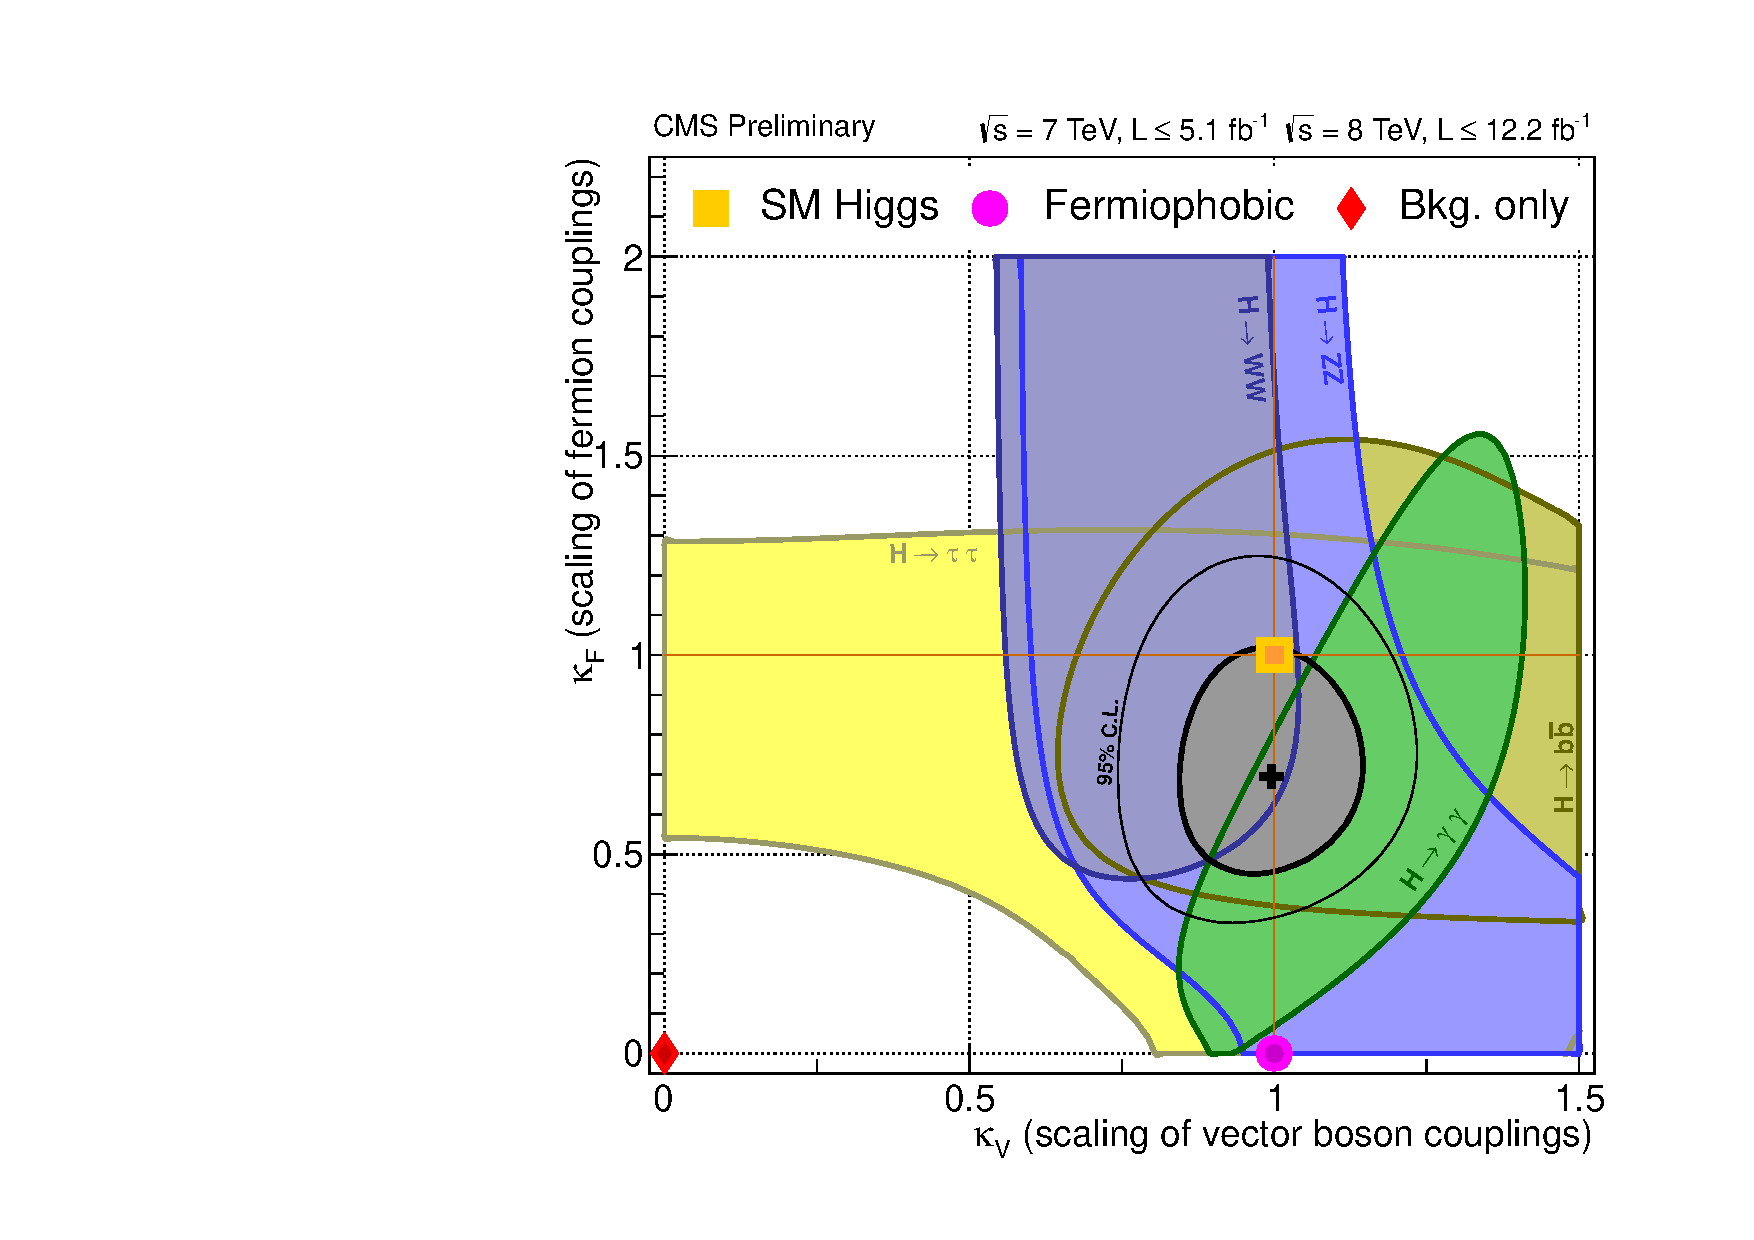
\includegraphics[width=.8\textwidth]{combinations/Figure_014-b.pdf}
\caption{The 68\% confidence contours extracted from data in the 
individual decay channels (coloured regions) and the full 
combination (solid line). The yellow square shows the SM value, while
the fermiophobic and background-only scenarios are indicated
by the pink dot and red diamond respectively.}
\label{fig:kvkf}
\end{figure}
